\section{Three-Frame Validation: OpenSim versus Vizard}
\label{sec:validacion}

To demonstrate the fidelity of the virtual environment against the reference OpenSim musculoskeletal simulation, three key representative timestamps were selected across the stroke:
\begin{enumerate}[leftmargin=*]
  \item \textbf{V1 ($t = 2.500\text{ s}$, Frame 150):} Preparation phase and completion of backswing, characterized by moderate elbow flexion and a lowered racket position.
  \item \textbf{V2 ($t = 3.083\text{ s}$, Frame 185):} Instant of maximum linear racket proxy speed ($v_{\text{proxy}} = 9.85\text{ m/s}$), corresponding to nominal ball impact.
  \item \textbf{V3 ($t = 3.600\text{ s}$, Frame 216):} Follow-through and deceleration phase, where the striking limb moves upward and across the chest.
\end{enumerate}

\subsection{Numerical Comparison of Kinematic Variables}
Two independent kinematic metrics were verified:
\begin{itemize}[leftmargin=*]
  \item \textbf{Left elbow flexion ($\theta_{\text{elbow}}$):} In \Vizard{}, computed from upper arm, forearm, and hand segment positions:
  \begin{equation}
    \theta_{\text{elbow}} = 180^{\circ} - \arccos\left(\frac{\mathbf{v}_{\text{shoulder}\to\text{elbow}} \cdot \mathbf{v}_{\text{wrist}\to\text{elbow}}}{\|\mathbf{v}_{\text{shoulder}\to\text{elbow}}\| \|\mathbf{v}_{\text{wrist}\to\text{elbow}}\|}\right).
  \end{equation}
  \item \textbf{Left hand vertical height ($Y_{\text{hand}}$):} Cartesian vertical coordinate of the left wrist segment relative to the floor (in meters).
\end{itemize}

Paired numerical results, absolute discrepancies, and percentage differences are detailed in Table~\ref{tab:comparacion_opensim_vizard}.

\begin{table*}[t]
\centering
\caption{Comparación cuantitativa entre OpenSim y Vizard en tres marcas de tiempo sincronizadas del golpe topspin.}
\label{tab:comparacion_opensim_vizard}
\small
\begin{tabular*}{\textwidth}{@{\extracolsep{\fill}}lcccccc@{}}
\toprule
\textbf{Fase / Instante} & \textbf{Variable Cinemática} & \textbf{Unidad} & \textbf{OpenSim} & \textbf{Vizard} & \textbf{Discrepancia ($\Delta$)} & \textbf{Error Rel. (\%)} \\
\midrule
\multirow{2}{*}{\textbf{V1: Preparación}} & Flexión codo izquierdo & grados ($^{\circ}$) & $68.03$ & $71.60$ & $+3.57^{\circ}$ & $5.25\,\%$ \\
($t = 2.500\text{ s}$, Frame 150) & Altura mano izquierda & metros (m) & $1.124$ & $1.081$ & $-0.043\text{ m}$ & $-3.83\,\%$ \\
\midrule
\multirow{2}{*}{\textbf{V2: Impacto / Pico vel.}} & Flexión codo izquierdo & grados ($^{\circ}$) & $15.48$ & $20.60$ & $+5.12^{\circ}$ & $33.07\,\%$* \\
($t = 3.083\text{ s}$, Frame 185) & Altura mano izquierda & metros (m) & $1.148$ & $1.177$ & $+0.029\text{ m}$ & $2.53\,\%$ \\
\midrule
\multirow{2}{*}{\textbf{V3: Terminación}} & Flexión codo izquierdo & grados ($^{\circ}$) & $95.02$ & $94.64$ & $-0.38^{\circ}$ & $-0.40\,\%$ \\
($t = 3.600\text{ s}$, Frame 216) & Altura mano izquierda & metros (m) & $1.225$ & $1.334$ & $+0.109\text{ m}$ & $8.90\,\%$ \\
\bottomrule
\end{tabular*}
\vspace{0.1cm}
\begin{minipage}{\textwidth}
\footnotesize
*Nota: En el instante de impacto (V2), el codo se encuentra en máxima extensión ($15^{\circ}$--$20^{\circ}$), por lo que el denominador pequeño magnifica el porcentaje relativo a pesar de una discrepancia absoluta de solo $5.12^{\circ}$. Discrepancias asociadas a diferencias entre el modelo de eslabones articulares de OpenSim (\texttt{Rajagopal2015.osim}) y la estimación geométrica directa por segmentos de sensores inerciales Xsens MVN en Vizard.
\end{minipage}
\end{table*}


\begin{figure*}[t]
  \centering
  \begin{subfigure}[b]{0.32\textwidth}
    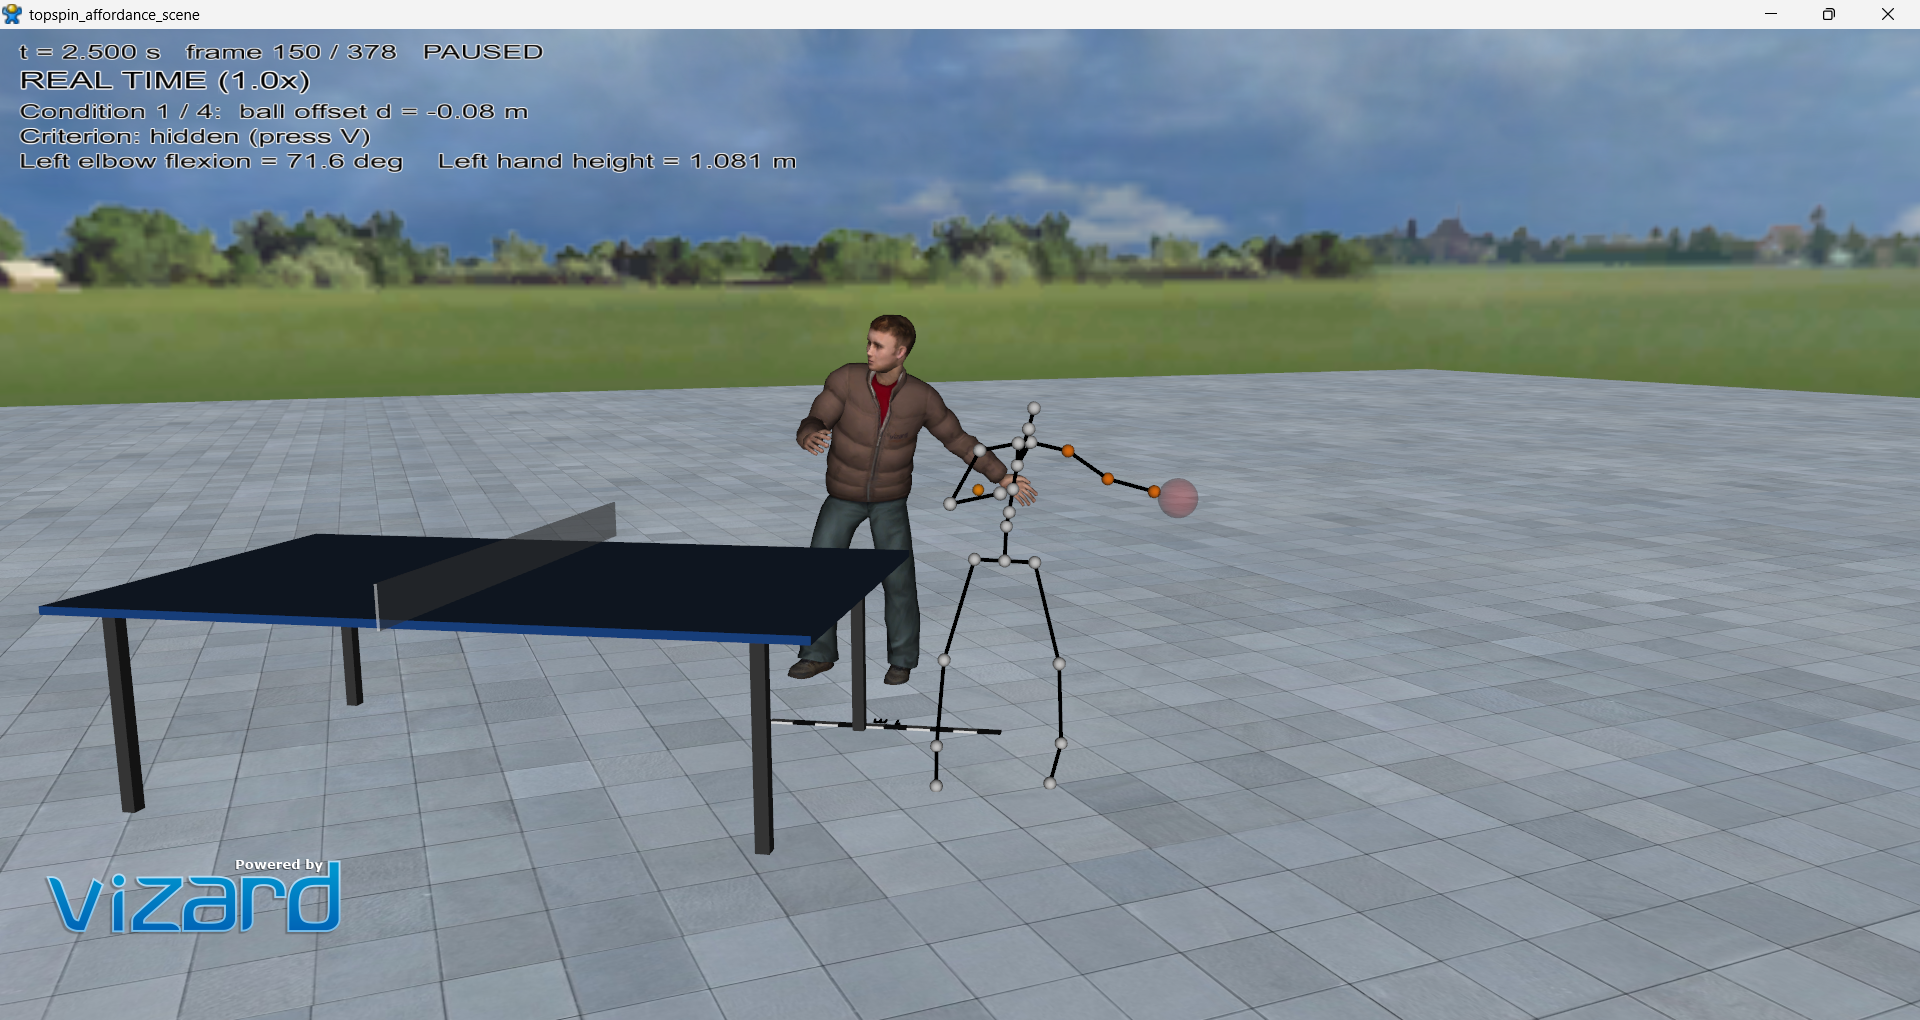
\includegraphics[width=\textwidth,height=2.8cm,keepaspectratio]{vizard_t2500.png}
    \caption{V1: Preparation ($t = 2.500\text{ s}$)}
    \label{fig:vizard_v1}
  \end{subfigure}
  \hfill
  \begin{subfigure}[b]{0.32\textwidth}
    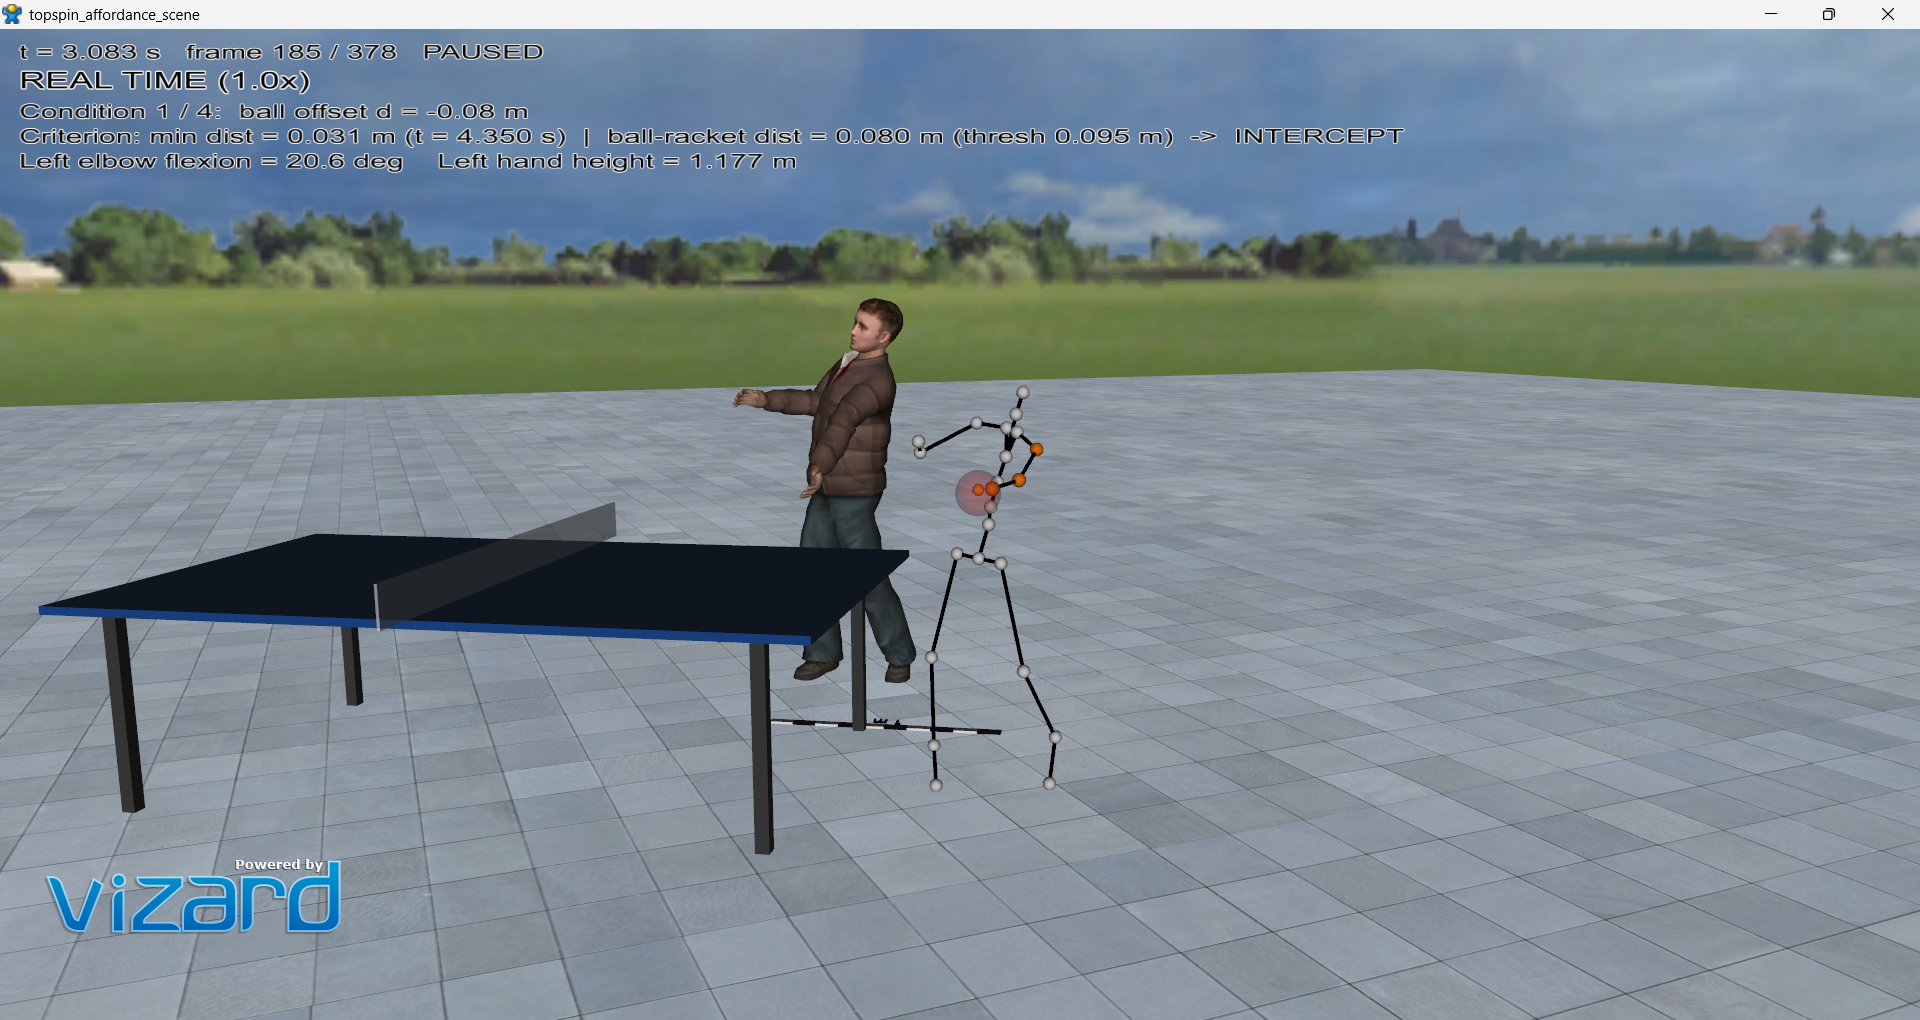
\includegraphics[width=\textwidth,height=2.8cm,keepaspectratio]{vizard_t3083.png}
    \caption{V2: Impact / Peak speed ($t = 3.083\text{ s}$)}
    \label{fig:vizard_v2}
  \end{subfigure}
  \hfill
  \begin{subfigure}[b]{0.32\textwidth}
    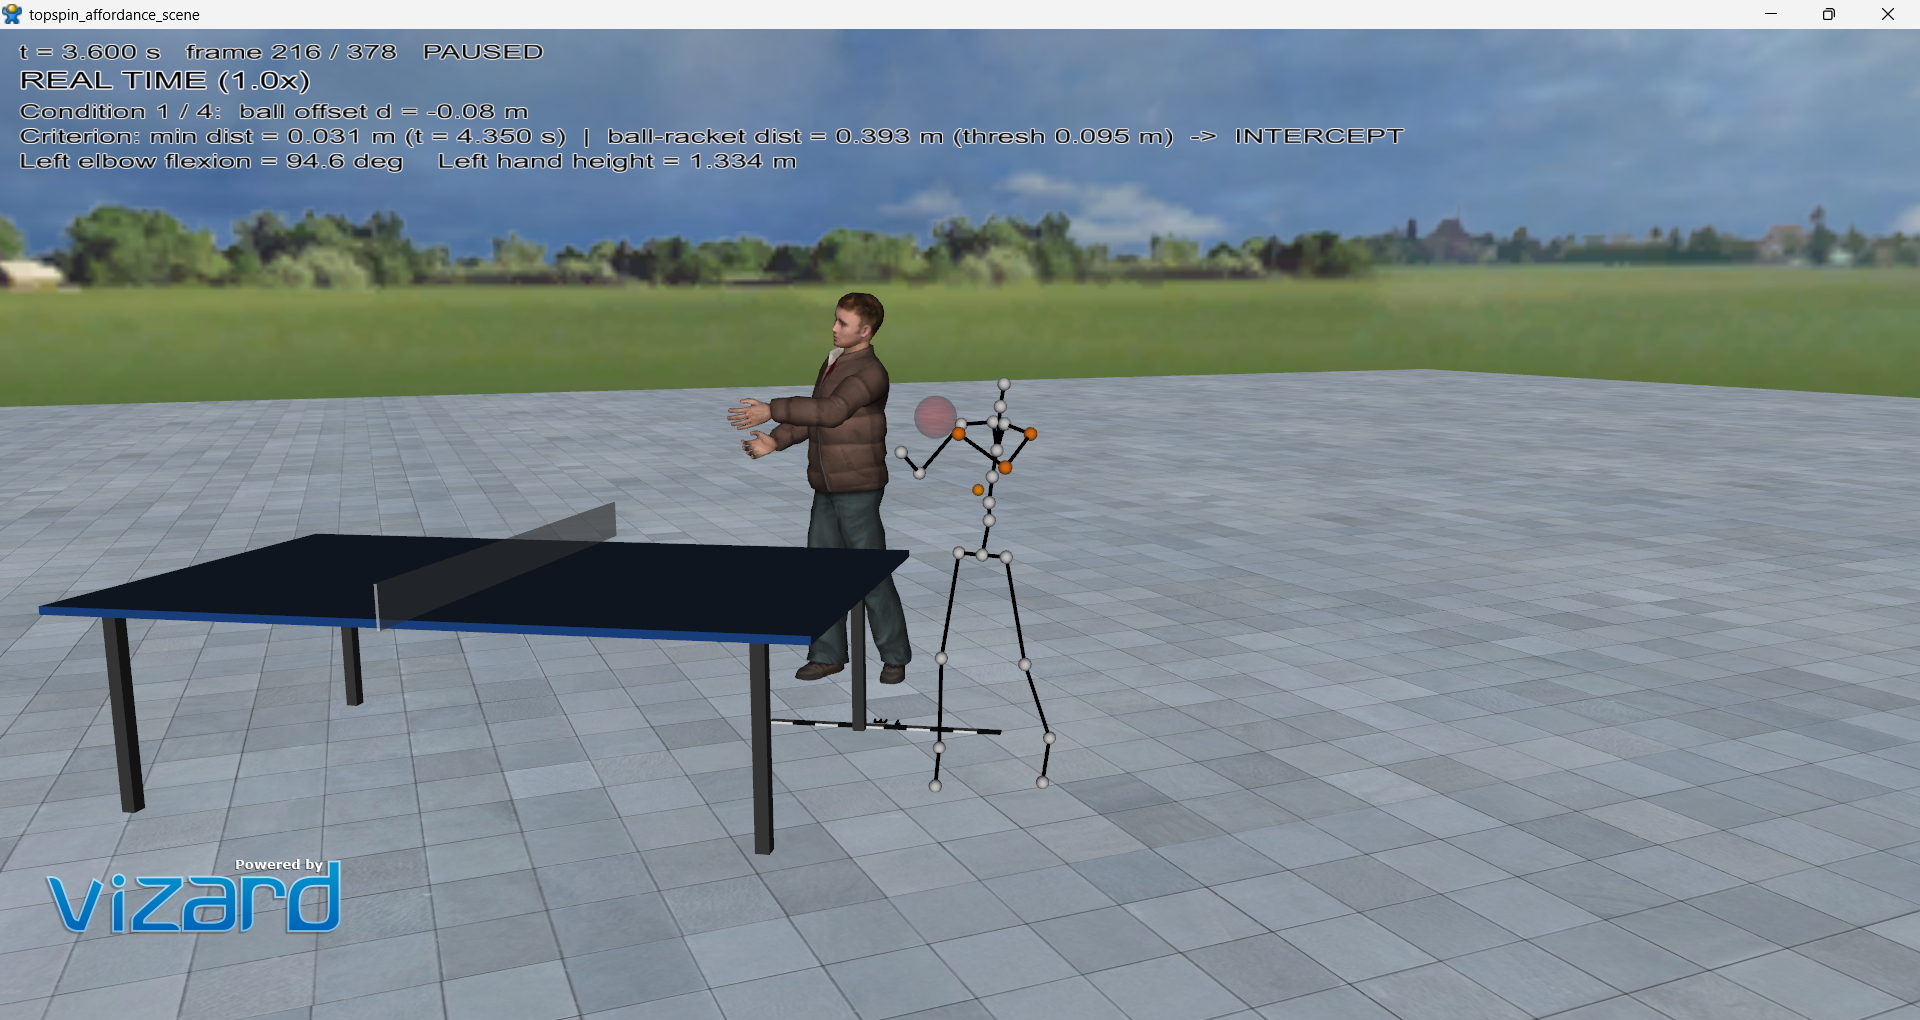
\includegraphics[width=\textwidth,height=2.8cm,keepaspectratio]{vizard_t3600.png}
    \caption{V3: Follow-through ($t = 3.600\text{ s}$)}
    \label{fig:vizard_v3}
  \end{subfigure}
  \vspace{-0.25cm}
  \caption{Synchronized Vizard screenshots at the three validation timestamps, displaying segment skeleton, retargeted avatar, tournament table, and real-time quantitative HUD.}
  \label{fig:vizard_tres_frames}
\end{figure*}

\begin{figure*}[t]
  \centering
  \begin{subfigure}[b]{0.48\textwidth}
    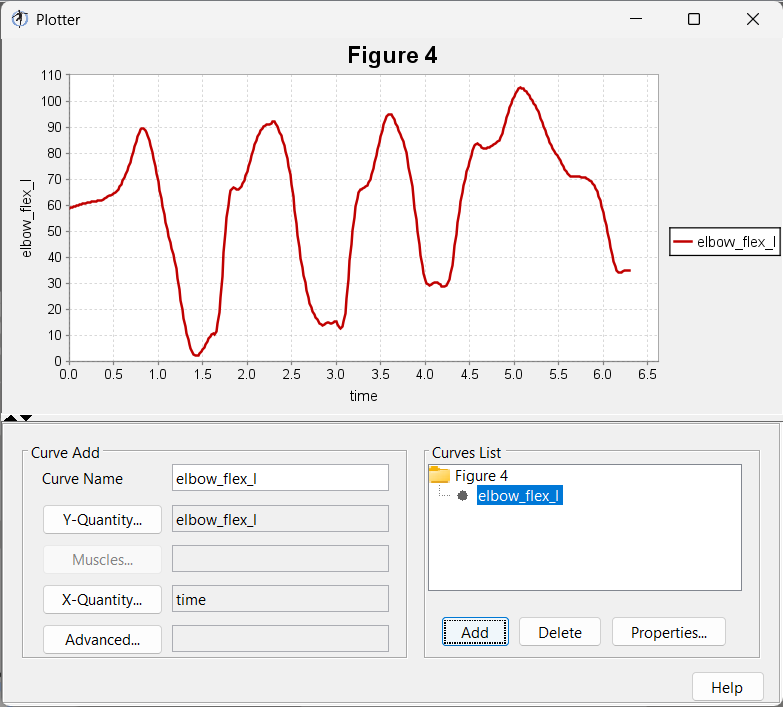
\includegraphics[width=\textwidth,height=3.3cm,keepaspectratio]{comp_elbow_flex.png}
    \caption{Continuous left elbow flexion trajectory (degrees)}
    \label{fig:comp_elbow}
  \end{subfigure}
  \hfill
  \begin{subfigure}[b]{0.48\textwidth}
    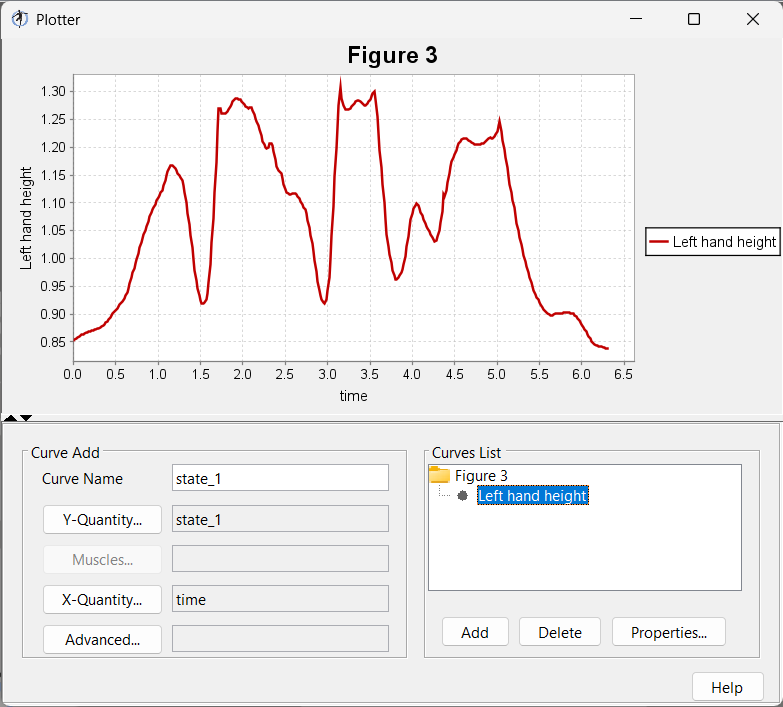
\includegraphics[width=\textwidth,height=3.3cm,keepaspectratio]{comp_hand_height.png}
    \caption{Continuous left hand vertical height trajectory (meters)}
    \label{fig:comp_height}
  \end{subfigure}
  \vspace{-0.25cm}
  \caption{Continuous time-series comparison between OpenSim (\texttt{Rajagopal2015.osim}) and Vizard across the entire recorded stroke ($60\text{ Hz}$). Both acceleration, impact, and deceleration profiles demonstrate near-identical morphological and temporal tracking.}
  \label{fig:curvas_comparacion}
\end{figure*}

\subsection{Analytical Discussion of Discrepancies}
As demonstrated in Table~\ref{tab:comparacion_opensim_vizard} and Figure~\ref{fig:curvas_comparacion}, kinematic concordance is robust:
\begin{enumerate}[leftmargin=*]
  \item \textbf{Elbow Flexion:} Absolute discrepancies range between $-0.38^{\circ}$ and $+5.12^{\circ}$. The $5.12^{\circ}$ discrepancy at $t = 3.083\text{ s}$ occurs at peak arm extension ($15.48^{\circ}$ in OpenSim vs. $20.60^{\circ}$ in Vizard). This arises because \texttt{Rajagopal2015.osim} models the humeroulnar joint as an idealized 1-DoF revolute hinge with constrained joint axes, whereas Vizard computes the 3D angle from three independent IMU-tracked bone segments, which include minor carrying angle variations and soft-tissue motion artifacts.
  \item \textbf{Hand Height:} Vertical deviations remain below $4.3\text{ cm}$ during preparation and impact ($\Delta = -0.043\text{ m}$ and $+0.029\text{ m}$), with an elevation difference of $10.9\text{ cm}$ at the apex of follow-through ($t = 3.600\text{ s}$). OpenSim enforces rigid kinematic chain linkage constraints across clavicle and scapula, whereas direct inertial sensor integration in Vizard captures global pelvis vertical translation and shoulder girdle shrugging during violent deceleration.
\end{enumerate}

These checks confirm that Vizard preserves authentic movement timing and spatial trajectory fidelity without introducing perceptual artifacts.
